\documentclass[11pt]{article}
\usepackage[utf8]{inputenc}	% Para caracteres en español
\usepackage{amsmath,amsthm,amsfonts,amssymb,amscd}
\usepackage{multirow,booktabs}
\usepackage[table]{xcolor}
\usepackage{fullpage}
\usepackage{lastpage}
\usepackage{enumitem}
\usepackage{fancyhdr}
\usepackage{mathrsfs}
\usepackage{wrapfig}
\usepackage{setspace}
\usepackage{calc}
\usepackage{multicol}
\usepackage{cancel}
\usepackage{float}
\usepackage{physics}
\usepackage[retainorgcmds]{IEEEtrantools}
\usepackage[margin=1cm]{geometry}
\usepackage{amsmath}
\newlength{\tabcont}
\setlength{\parindent}{0.0in}
\setlength{\parskip}{0.05in}
\usepackage{empheq}
\usepackage{framed}
\usepackage[most]{tcolorbox}
\usepackage{xcolor}
\usepackage[version=3]{mhchem}
\usepackage[english]{babel}
\usepackage[utf8]{inputenc}
\usepackage{graphicx}
\usepackage[colorinlistoftodos]{todonotes}

\colorlet{shadecolor}{orange!15}
\parindent 0in
\parskip 12pt
\geometry{margin=1in, headsep=0.25in}
\theoremstyle{definition}
\newtheorem{defn}{Definition}
\newtheorem{reg}{Rule}
\newtheorem{exer}{Exercise}
\newtheorem{note}{Note}
\begin{document}
\setcounter{section}{2}
%\setcounter{subsection}{}
\title{Problem Set 4}

%==============================================================
%\thispagestyle{empty}

\begin{center}
{\LARGE \bf Problem Set 4}\\
{\large Physics 180}\\
Olyn D. Desabelle
\end{center}

\begin{figure}[h!]
    \centering
    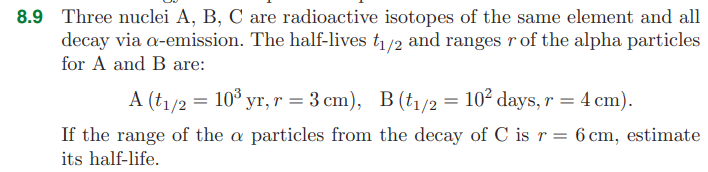
\includegraphics[scale = 0.5]{8.9.png}
\end{figure}

We will be using the Geiger–Nuttall relation to get the half-life of the $C$ isotope:

\begin{align}
    \log_{10} \lambda = c + d \log_{10} r 
\end{align}

where $\lambda = \frac{\ln 2}{t_{1/2}}$. We begin with finding the values of $c$ and $d$ using the given for the $A$ and $B$ isotopes with:

\begin{align}
        \log_{10} \left(\frac{\ln 2}{t_{1/2}} \right) = c + d \log_{10} r 
\end{align}

converting them to similar units, we have the system of equations:

\begin{align}
    \log_{10} \left(\frac{\ln 2}{525 \; 948\; 766\; \text{min}} \right) &= c + d \log_{10}(3\; \text{cm}) \\
    \log_{10} \left(\frac{\ln 2}{144\; 000\; \text{min}} \right) &= c + d \log_{10}(4\; \text{cm})\\
    %-8.88 &= c+d(0.48)\\
    %-5.32 &= c+d(0.60)
\end{align}

we can solve these using substitution:

\begin{align}
    c &=  \log_{10} \left(\frac{\ln 2}{525 \; 948\; 766\; \text{min}} \right) -  d \log_{10}(3\; \text{cm})\\
    \log_{10} \left(\frac{\ln 2}{144\; 000\; \text{min}} \right) &= \log_{10} \left(\frac{\ln 2}{525 \; 948\; 766\; \text{min}} \right) -  d \log_{10}(3\; \text{cm}) + d \log_{10}(4\; \text{cm})\\
    d &=  \left[\log_{10}\left(\frac{\ln 2}{525 \; 948\; 766\; \text{min}} \right) - \log_{10} \left(\frac{\ln 2}{144\; 000\; \text{min}} \right)\right] \left[\frac{1}{\log_{10}(3\; \text{cm}) - \log_{10}(4\; \text{cm})}\right]
\end{align}

from here we get the following values:

\begin{align}
    c &= -22.49 \\
    d &= 28.51 
\end{align}

getting the half-life for the $C$ isotope:

\begin{align}
    10^{\log_{10}(\ln 2) -c - d \log_{10} r}  &= t_{1/2}\\
    10^{\log_{10}(\ln 2) + 22.49 - 28.51 \log_{10}(6)}  &= t_{1/2}
\end{align}

\begin{equation}
\boxed{
    t_{1/2} = 1.37\;\text{min}
}
\end{equation}
%==============================================================
\newpage
%==============================================================

\begin{figure}[h!]
    \centering
    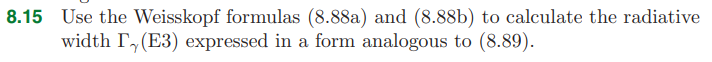
\includegraphics[scale = 0.55]{8.15.png}
\end{figure}

The emission rate $T_{fi}^{E,M}$ is given by:

\begin{align}
    T_{fi}^{E,M} &= \frac{1}{4\pi\epsilon_0} \frac{8\pi (L+1)}{L[(2L+1)!!]^2} \frac{1}{\hbar} \left(\frac{E_{\gamma}}{\hbar c}\right)^{2L+1} B_{fi}^{E,M}(L)
\end{align}

in this case, we only need $B_{fi}^{E,M}(L) = B^E (L)$ for the E3 multipole transition. The reduced transition probability for electric radiation ($B^E (L)$) is given by:

\begin{align}
    B^E (L) &= \frac{e^2}{4\pi} \left(\frac{3}{L+3}\right)^2 (R_0)^{2L} A^{2L/3}\\
\end{align}

For E3 multipole transition ($L=3$), we then have $B^E (L)$ as:

\begin{align}
    B^E (L=3) &= \frac{e^2}{4\pi} \left(\frac{1}{2}\right)^2 (R_0)^{6} A^{2}\\
    B^E (3) &= \frac{e^2}{16\pi}R_0^{6} A^{2}
\end{align}

using this for $T_{fi}^{E,M}$:

\begin{align}
    T^{E} &= \frac{1}{4\pi\epsilon_0} 
    \frac{8\pi (4)}{3[(7)!!]^2} 
    \frac{1}{\hbar} 
    \left(\frac{E_{\gamma}}{\hbar c}\right)^{7}
     B^{E}(3)\\
    T^{E} &= \frac{1}{\epsilon_0} 
    \frac{8}{3[(7)!!]^2} 
    \frac{1}{\hbar} 
    \left(\frac{E_{\gamma}}{\hbar c}\right)^{7}
     B^{E}(3)
\end{align}

we note that for the double factorial for odd integers, we have:

\begin{align}
    (2n+1)!! &= \frac{(2n+1)!}{2^n n!}\\
    (7)!! &= \frac{(7)!}{2^3 (3!)} = 105\\
\end{align}


going back to the emission rate, we have:

\begin{align}
    T^{E} &= \frac{1}{\epsilon_0} 
    \frac{8}{3[105
    ]^2} 
    \frac{1}{\hbar} 
    \left(\frac{E_{\gamma}}{\hbar c}\right)^{7}
     \left(\frac{e^2}{16\pi}R_0^{6} A^{2}\right)\\
     &=
     \frac{e^2 R_0^6}
     {6\pi[105
     ]^2\epsilon_0 \hbar^8 c^7}
     E_{\gamma}^7
     A^2\\
     &=
     \frac{e^2 (1.21\; \text{fm})^6}
     {6\pi[105
     ]^2(55.263\; e^2 \text{GeV}^{-1}\text{fm}^{-1}) (6.582\cross 10^{−25}\; \text{GeV s})^8 (3\cross 10^{23}\; \text{fm/s})^7}
     E_{\gamma}^7
     A^2\\
\end{align}


to get the radiative width $\Gamma$, we use:

\begin{align}
    \Gamma &= \hbar T^E\\
    &= \frac{e^2 (1.21\; \text{fm})^6}
    {6\pi[105
    ]^2(55.263\; e^2 \text{GeV}^{-1}\text{fm}^{-1}) (6.582\cross 10^{−25}\; \text{GeV s})^7 (3\cross 10^{23}\; \text{fm/s})^7}
    E_{\gamma}^7
    A^2\\
\end{align}
% e = 1.60218 × 10−19 C
% c = 2.99792 × 10^8 m s−1 
% epsilon_0 = 55.26349406	e2⋅GeV−1⋅fm−1
% R_0 = 1.21 fm
% hbar = 6.58212 × 10−25 GeV s
% c = 2.99792458e+23 fm/s

\begin{equation}
\boxed{
    \Gamma = (2.346 \cross 10^{16})E_{\gamma}^7 
    A^2 \; \text{eV}
}
\end{equation}
%==================================
\end{document}